\documentclass[12pt]{article}

\renewcommand*\familydefault{\sfdefault}

\usepackage[left=1in,right=1in,top=1in,bottom=1in]{geometry}
\usepackage{graphics,epsfig,graphicx,float,subfigure,color}
\usepackage{algorithm,algorithmic}
\usepackage{amsmath,amssymb,amsbsy,amsfonts,amsthm}
\usepackage{listings}
\usepackage{color} %red, green, blue, yellow, cyan, magenta, black, white

\title{Snailgate: Summary of Physics}

\begin{document}

\maketitle

\section{Introduction}
Figure~\ref{fig:system} shows a summary of forces acting on the system. Note that here we do not add the Normal force on the vertices touching the ground.
\begin{figure}[hbt]
  \begin{center}
    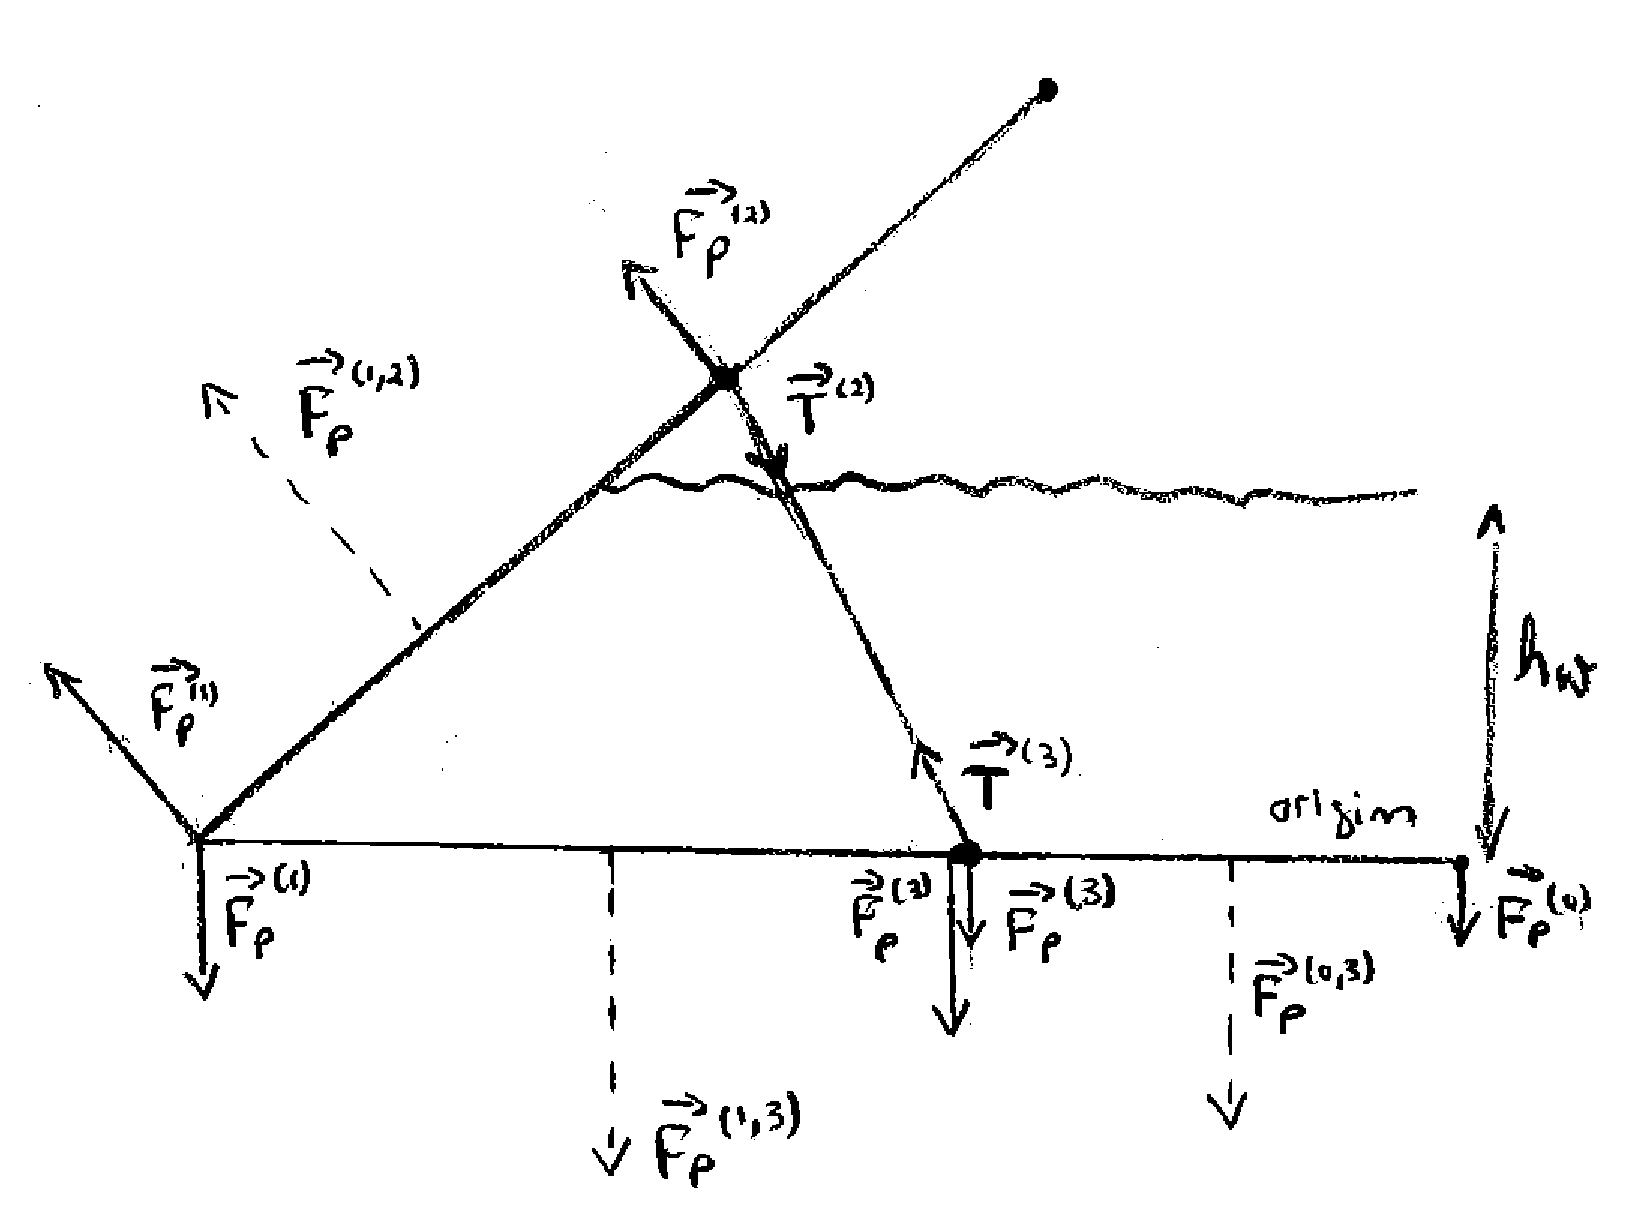
\includegraphics[width=0.8\textwidth]{system.png}
  \end{center}
  \caption{Watergate system.}
  \label{fig:system}
\end{figure}

Note that this is a 2D representation of a 3D system. To be able to simulate this, we consider that the watergate has a fixed width equal to $W$, like shown in Figure~\ref{fig:3D}.
\begin{figure}[hbt]
  \begin{center}
    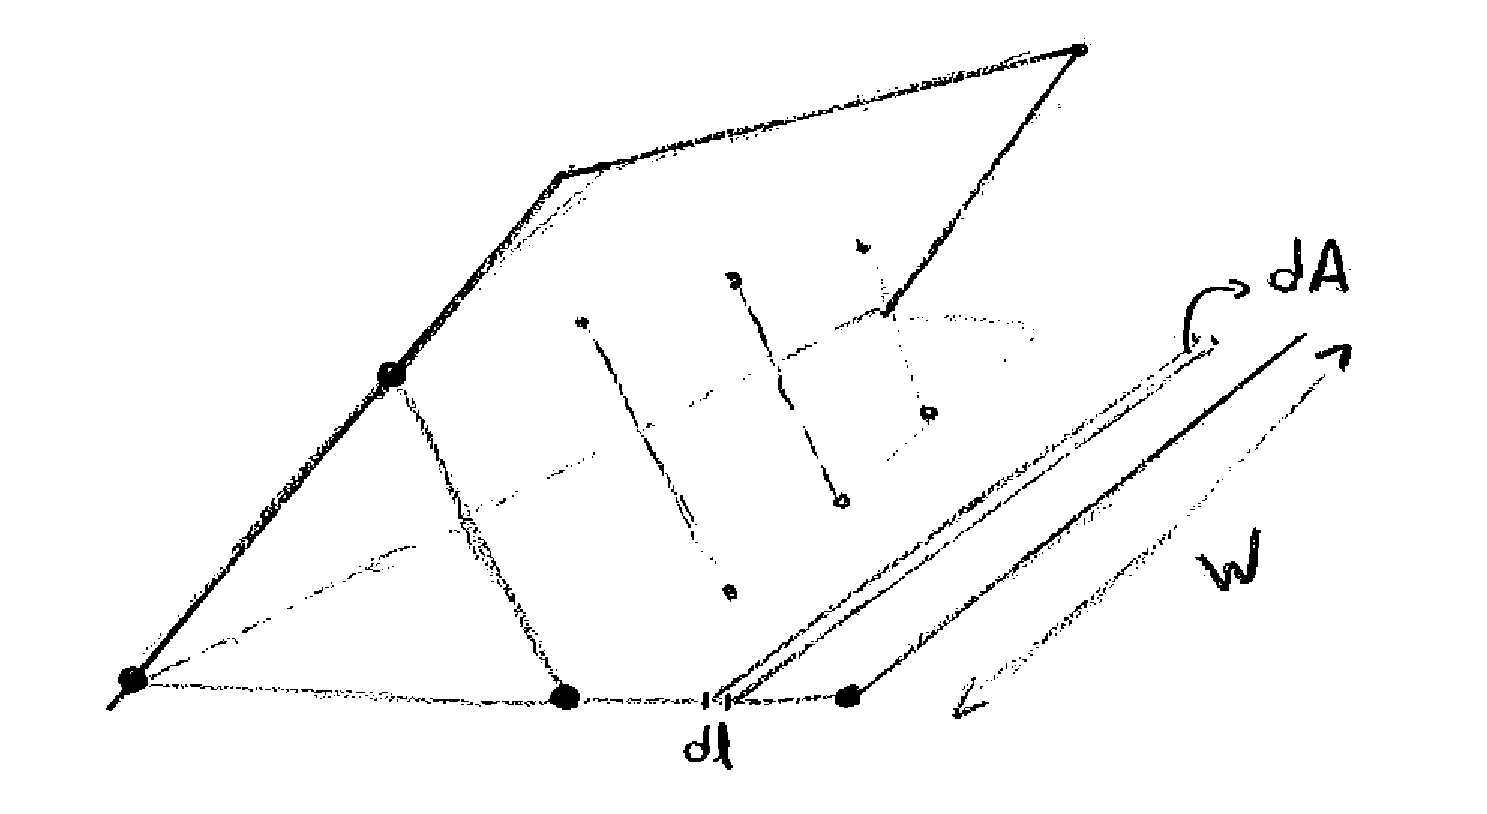
\includegraphics[width=0.8\textwidth]{3D.png}
  \end{center}
  \caption{3D picture of watergate.}
  \label{fig:3D}
\end{figure}

\section{Water Pressure Forces}

First, let's discuss about the force on each node arising from water pressure. Let's call these forces $F_P^{(i,j)}$, where $(i,j)$ represent the edge where the force is being applied. We know that the pressure can be computed as follows:
\begin{align*}
  P_w = \rho g (h_w - y) \text{, for $h_w > y$ }  
\end{align*}
where $\rho (kg/m^3)$ is the density of water, $g (m/s^2)$ is the gravity, $h_w (m)$ is the height of water in the snailgate (measured from the origin) and $y$ is the vertical coordinate of the current point where the pressure is being measured. Here, we can consider the water density as $\rho = 1 kg/m^3$ and the gravity as $g = 9.81 m/s^2$. Notice that the unit of pressure is then $N/m^2$ or $Pa$ (Pascal).

Observe that the formula is only valid for points under the water and that we are not considering here the atmosphere pressure. The total force in each point should be $P_{\text{atm}} + P_w$. But since the forces will arise from the difference of pressure, we can discard $P_{\text{atm}}$ in our analysis.

Let's think then how a \emph{water pressure force} in an edge (bar) can be computed.

\subsection{Force in infinitesimal area}
Let's consider the force caused by pressure in an infinitesimal length of the watergate border. We can write
\begin{align*}
  dF_P &= P_w dA\\
  &=  \rho g (h_w - y) W dl
\end{align*}
where $dl$ is the infinitesimal length in the bar, as shown in Figure~\ref{fig:diagonal}.

\subsection{General formula for force}
We can then integrate the force in the entire edge to discover its resultant force.
\begin{align*}
  F_P &= \int dF_P = \int P_w dA\\
  &= \int \rho g (h_w - y) W dl\\
  &= \rho g W \int (h_w - y) dl
\end{align*}

Note that we cannot consider $y$ constant in this case, since it can be related to $l$ (distance from $v_i$ to current point), as in the case of edges in diagonal position inside the water. See Figure~\ref{fig:diagonal}. However, we know:
\begin{align*}
  (dx)^2 + (dy)^2 = (dl)^2\\
  dl = dy/\sin \theta
\end{align*} 
where $\theta$ is the angle between the edge and the horizontal axis.

\begin{figure}[hbt]
  \begin{center}
    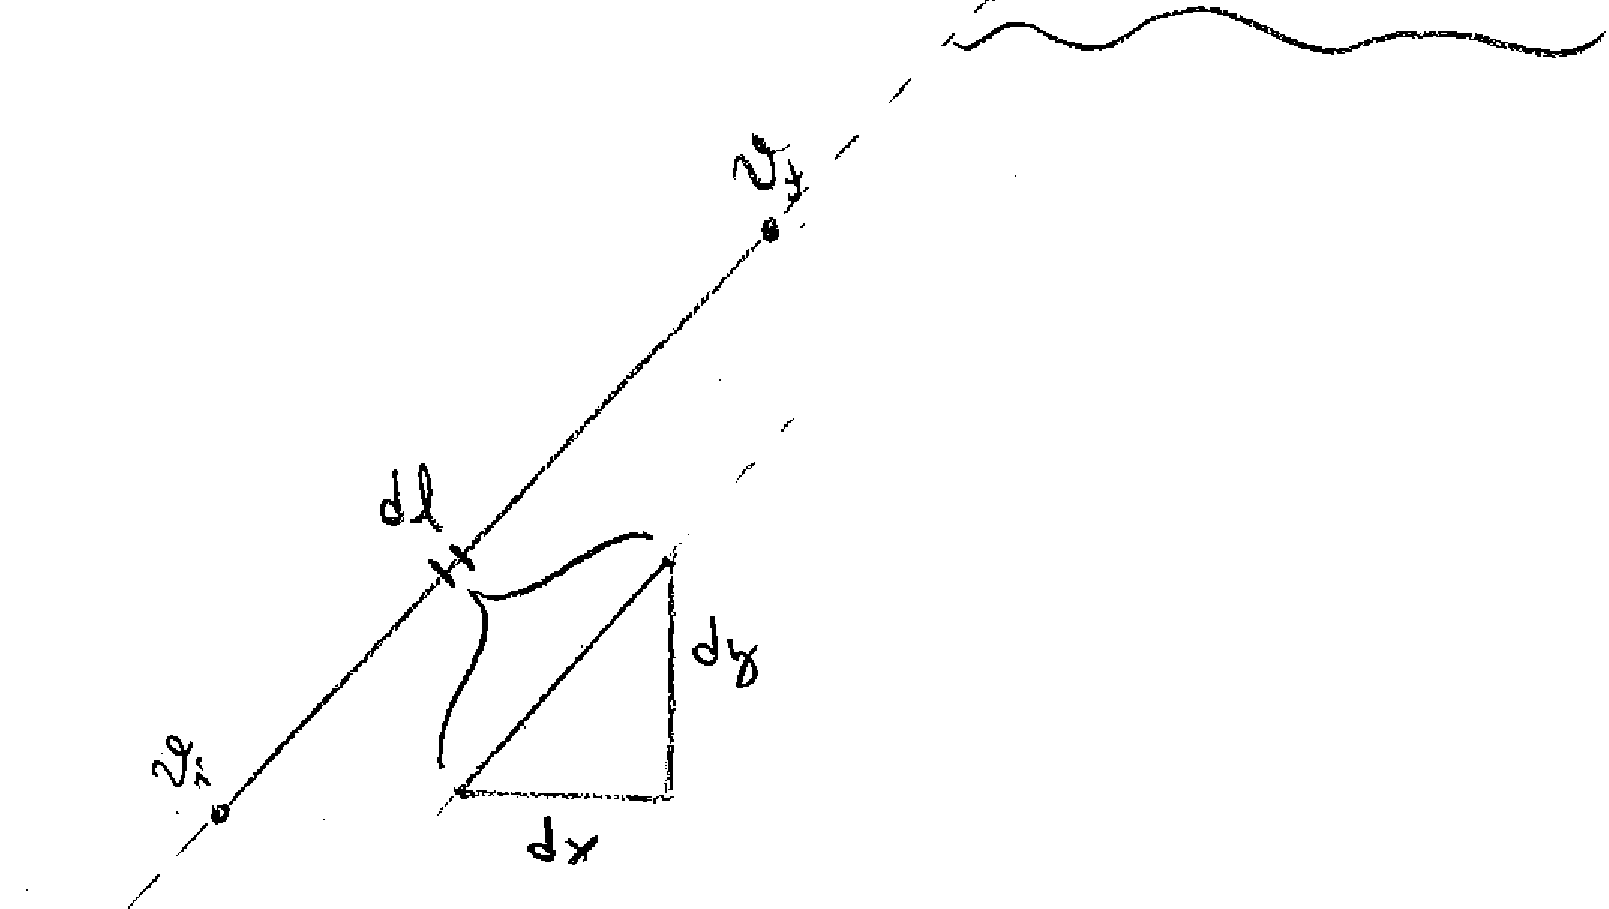
\includegraphics[width=0.8\textwidth]{diagonal.png}
  \end{center}
  \caption{Diagonal edge (bar) inside water.}
  \label{fig:diagonal}
\end{figure}

Since $\theta$ is constant for a straight edge, we can write:
\begin{align*}
  F_P &= \rho g W \int (h_w - y) dl\\
  &= \rho g W \int (h_w - y) dy/\sin{\theta}\\
  &= \frac{\rho g W}{\sin{\theta}} \left[ y \left(h_w - \frac{y}{2}\right) \right]_{y_i}^{y_j}
\end{align*}

Now, let's present some special cases, as shown in Figure~\ref{fig:horizontal-vertical}.

\begin{figure}[hbt]
  \begin{center}
    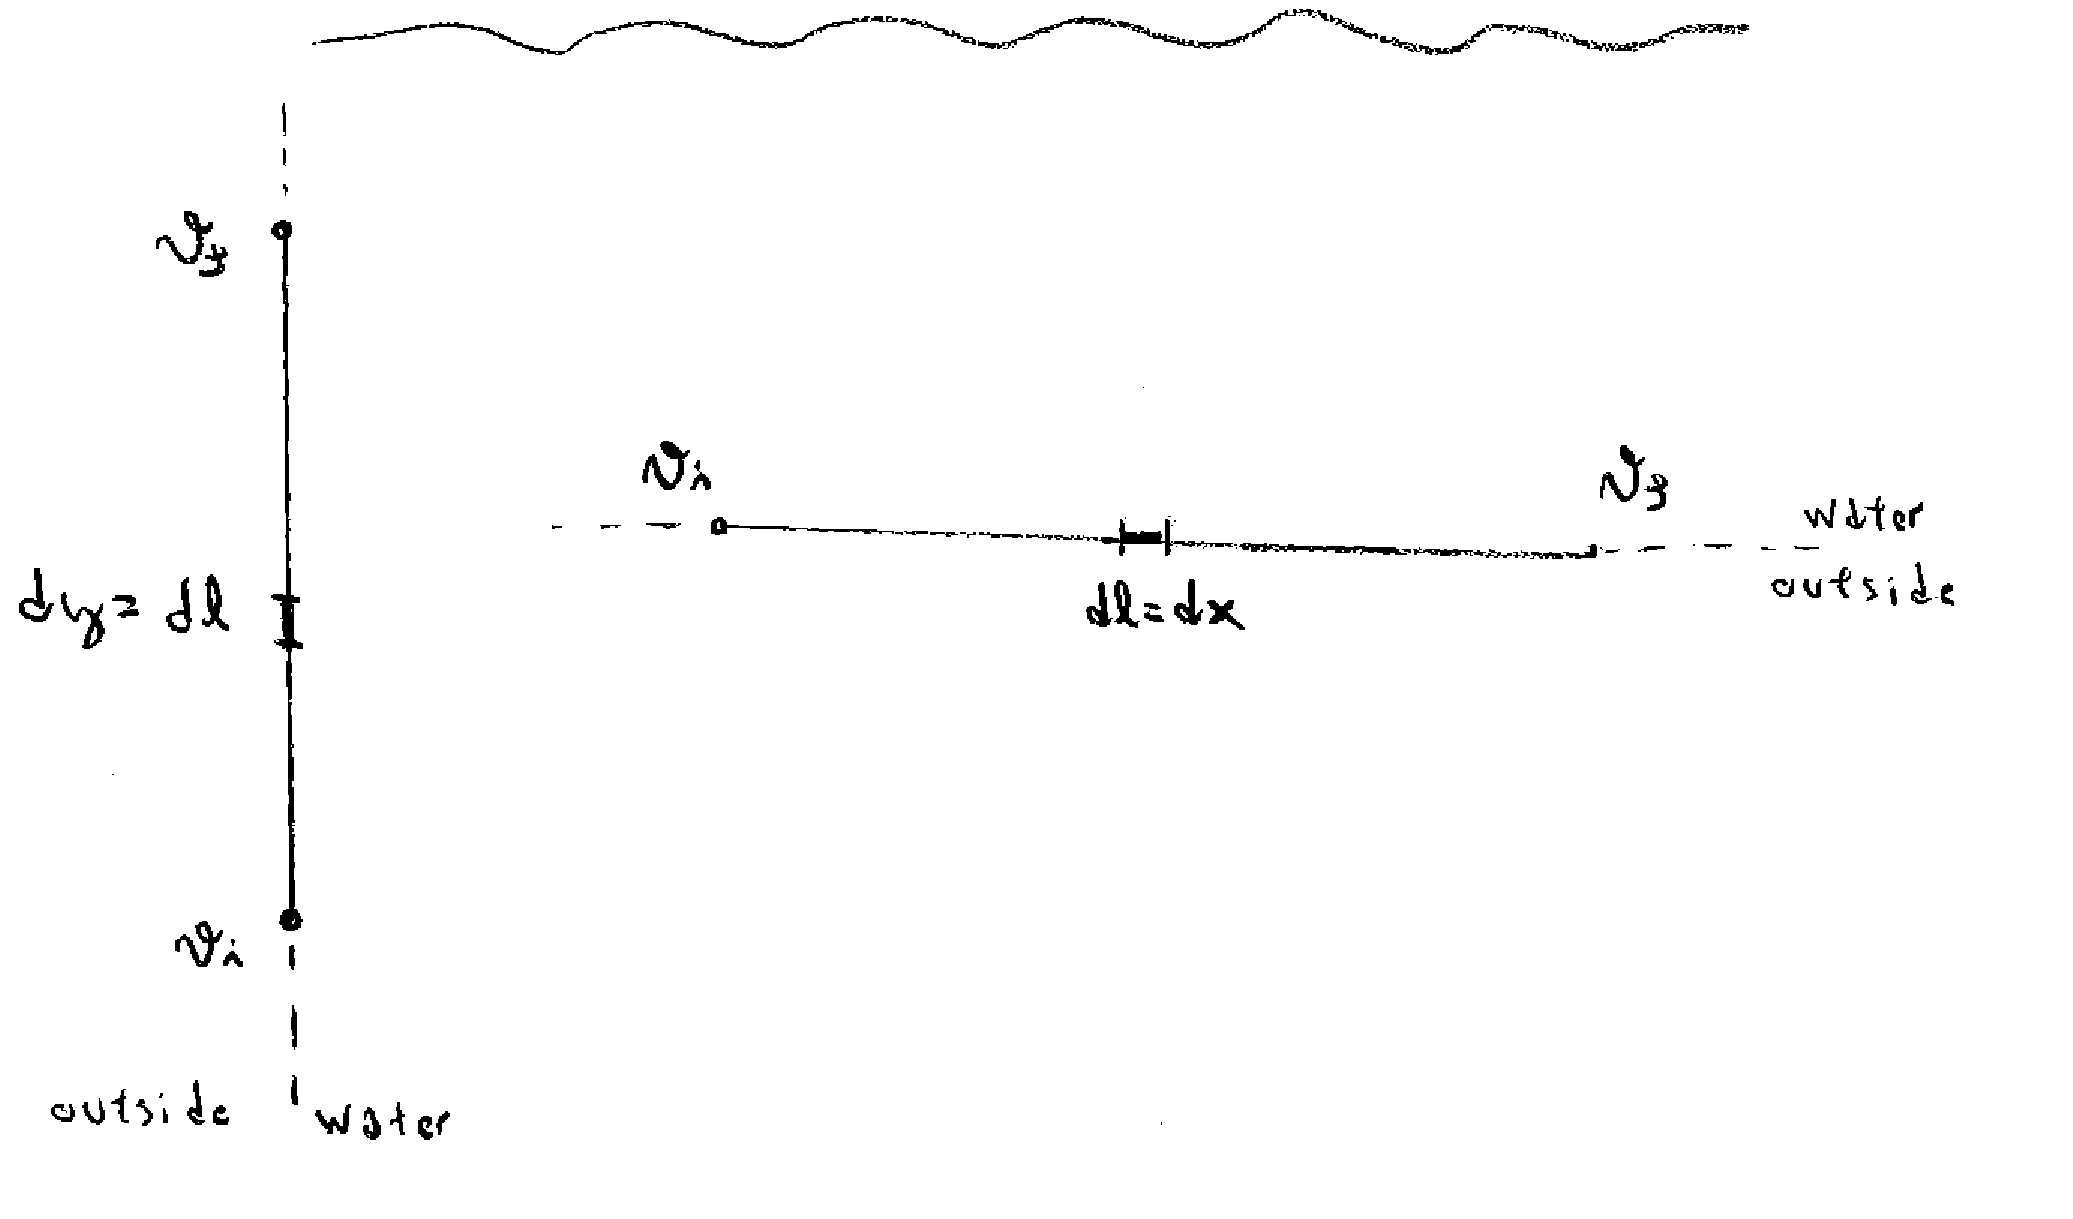
\includegraphics[width=0.8\textwidth]{horizontal-vertical.png}
  \end{center}
  \caption{Special cases: vertical (left); horizontal (right) }
  \label{fig:horizontal-vertical}
\end{figure}

\subsection{Force in a vertical bar in water}
In the case of a vertical bar in the water, we know $\theta = \pi/4$ and $\sin\theta = 1$. Then, the force is simply:
\begin{align*}
  F_P &= \rho g W \left[ y \left(h_w - \frac{y}{2} \right) \right]_{y_i}^{y_j}
\end{align*}

\subsection{Force in a horizontal bar in water}
Consider a bar in horizontal position immerse in water. In this case, we know $y_i = y_j = y$ is constant. Then the pressure in each point of the bar is constant and equal to $\rho g (h_w - y)$. We can obtain the total force in the bar by simply integrating the force acting on each infinitesimal length $dl = dx$ of the bar. 
\begin{align*}
  dF_P &= P_w dA \\
  F_P &= \int dF_P = \int P_w dA\\
  &= \int \rho g (h_w - y) W dl\\
  &= \rho g (h_w - y) W \int_{x_i}^{x_j}  dx\\
  &= \rho g W (h_w - y) \Delta x
\end{align*}

\section{Tension forces}
In our model, we also consider the possibility of a rope between two vertices of the system. When the rope is stretched, it gives a force in the opposite direction of the strain:
\begin{align*}
  T = -k \Delta L = -k (L - L_0)
\end{align*}
where $k$ is the elasticity tensor (spring constant of Hooke's law) of the rope.
Also, $L$ can be described as follows:
\begin{align*}
L = 
\begin{cases}
    L_0,& \text{if } d(i,j) < L_0\\
    d(i,j),              & \text{otherwise}
\end{cases}
\end{align*}
where $d(i,j) = \left[ (x_j-x_i)^2 + (y_j - y_i)^2 \right]^{1/2}$.

Notice that the force will be different than $0$ only if the rope is being stretched.

\section{Other forces}
All vertices in contact with the floor of the system, will have a normal force keeping them in equilibrium with respect to the vertical forces. This vertices will be tagged as fixed for the simulation.

In addition, there may be other forces acting on the system, depending on how complex is our model. 



\section{Resulting Forces}
\label{sec:center-of-load}

Recall that $F_P$ corresponds to the magnitude of pressure forces on the edge. However, it is important to know how to determine a single resultant force vector in the edge that represents $F_p$. We can do this by computing the centroid of load for each coordinate. For the vertical axis, this is easy:
\begin{align*}
  \bar y &= \frac{\int y dF_P(y)}{\int dF_p}\\
  &= \frac{\rho g W \left[ y^2 (h_w/2 - y/3)\right]_{y_i}^{y_j}}{\rho g W \left[ y (h_w - y/2) \right]_{y_i}^{y_j}}\\
  &= \frac{\left[ y^2 (h_w/2 - y/3)\right]_{y_i}^{y_j}}{\left[ y (h_w - y/2) \right]_{y_i}^{y_j}}
\end{align*}

After obtaining $\bar y$, it is easy to find $\bar x$.

Figure~\ref{fig:distributed-load} shows the resulting force of the system, given that the load varies with height.
\begin{figure}[hbt]
  \begin{center}
    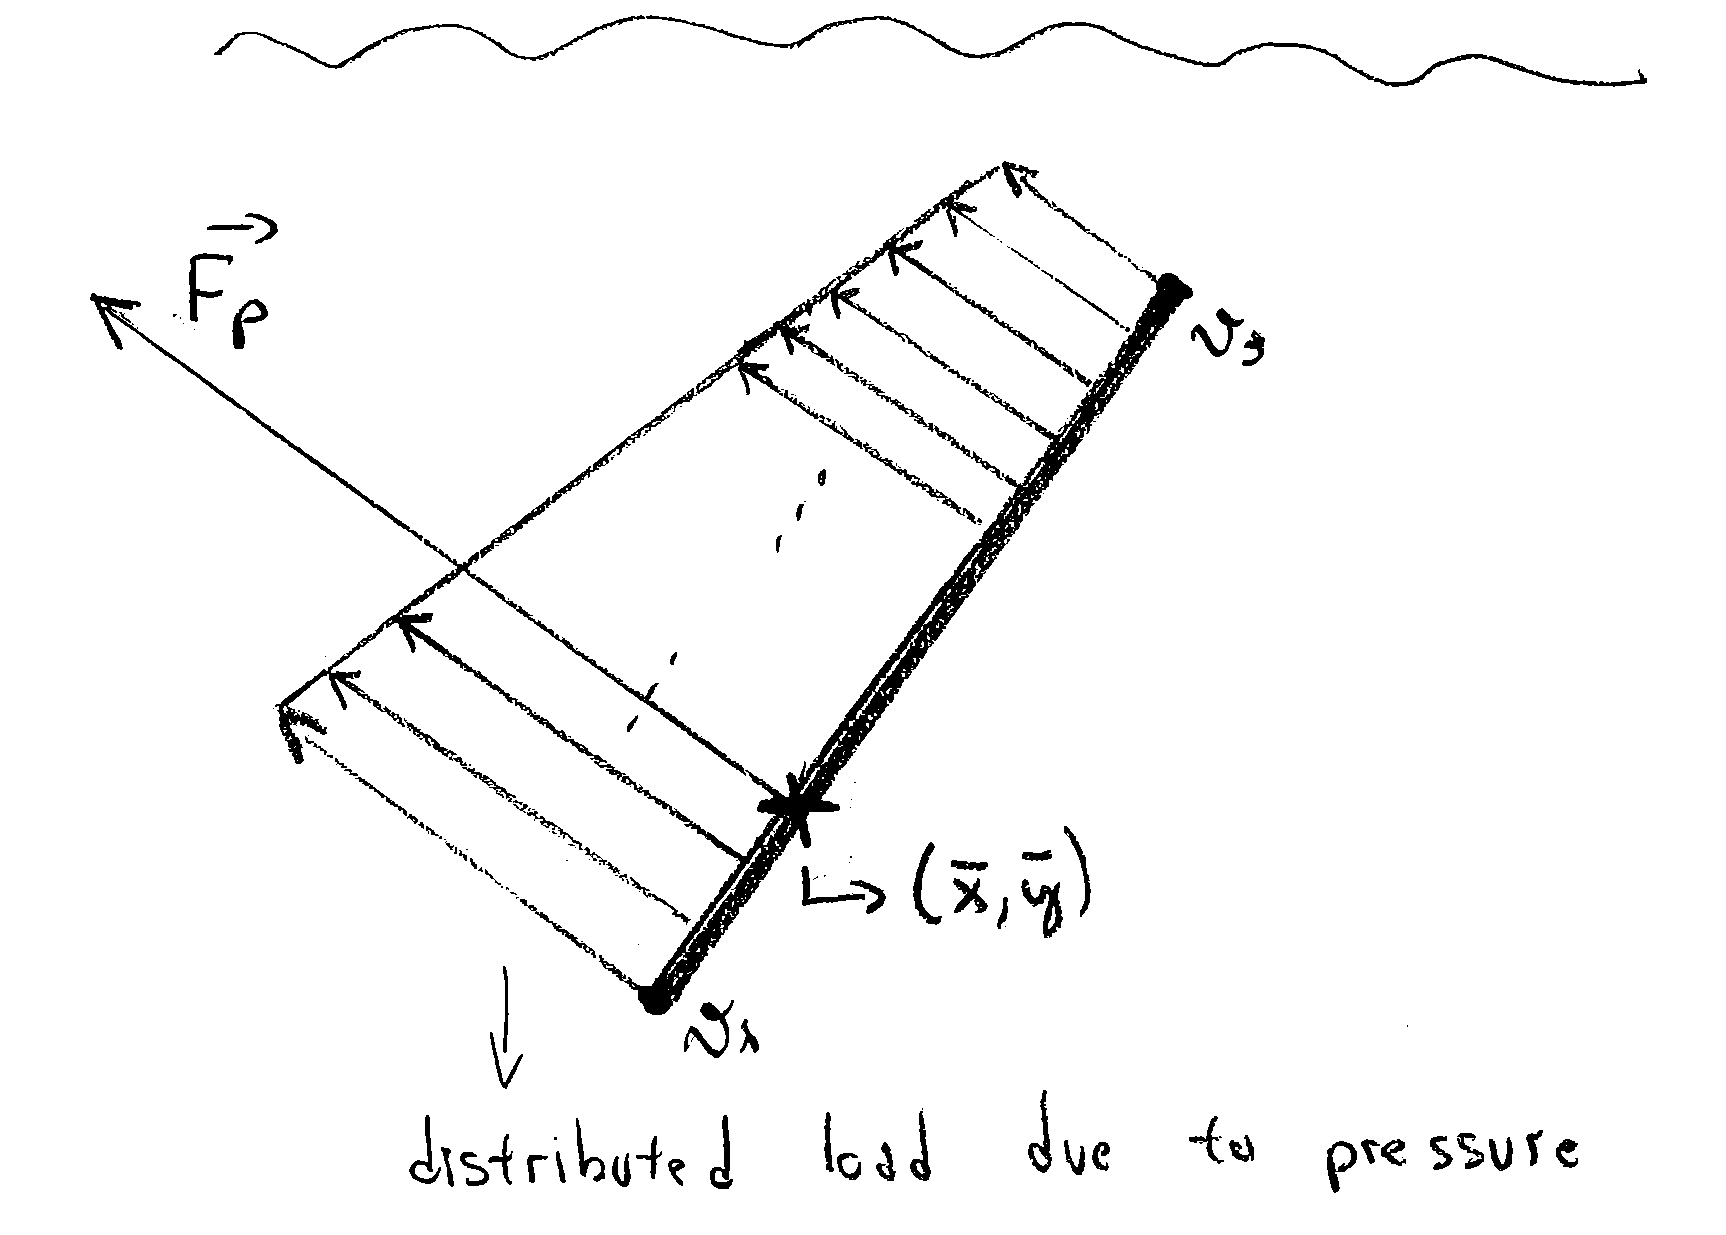
\includegraphics[width=0.8\textwidth]{distributed-load.png}
  \end{center}
  \caption{Distributed load and resulting force.}
  \label{fig:distributed-load}
\end{figure}

\subsection{Edge forces to vertex forces}

To better represent the forces in the nodes of the watergate system, we should compute the corresponding forces on the vertices in such a way that they sum up to the resulting force. There are different ideas on how to reach this:

\begin{enumerate}
  \item \textbf{Split forces:} simply use half of the force on each node.
  \item \textbf{Split edge:} split the edge in half and assign to each vertex (of the original edge) the force associated with the splitted edge incident to it.
  \item \textbf{Weighted forces:} weight the forces using the known location of the Resultant force on the edge, as explained in Section~\ref{sec:center-of-load}. This can be done in such a way that the two forces (one for each vertex) produce the same final torque as the one produced by the resulting force $F_p$. This idea is shown in Figure~\ref{fig:vertex-forces}.
\end{enumerate}

\begin{figure}[hbt]
  \begin{center}
    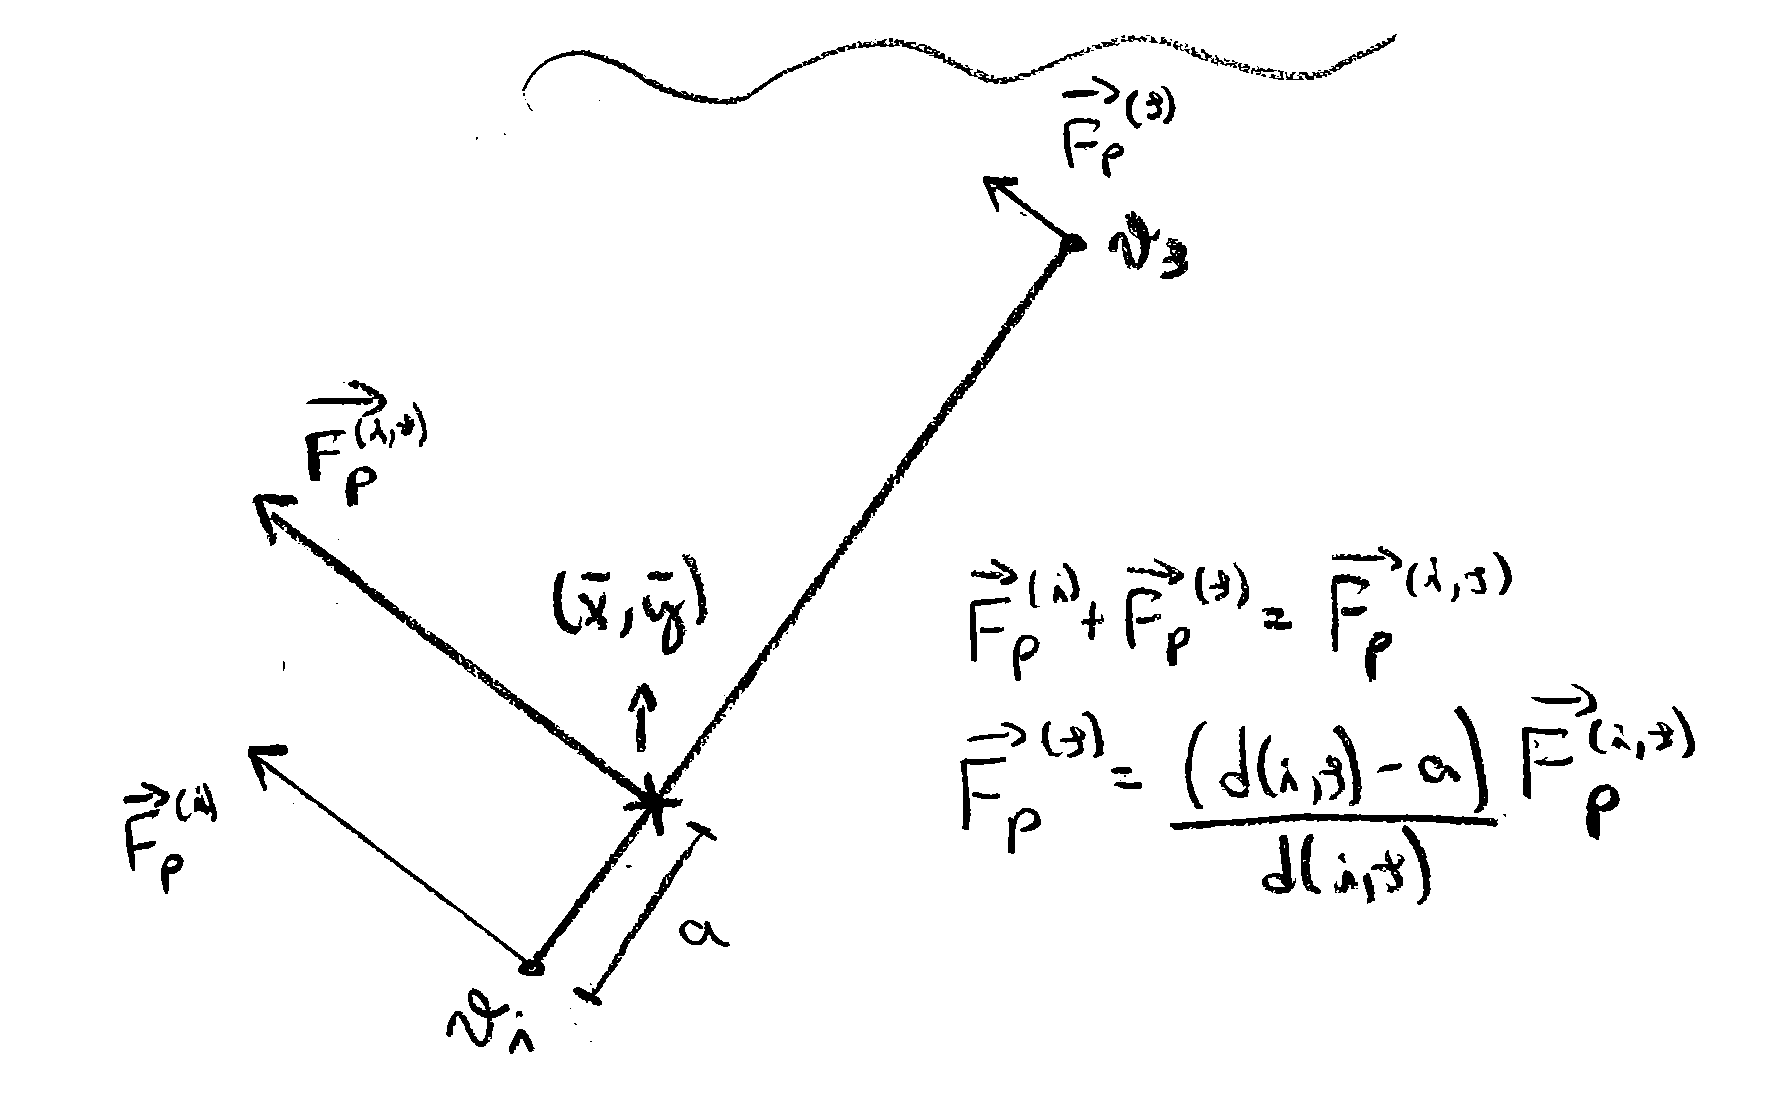
\includegraphics[width=0.8\textwidth]{vertex-forces.png}
  \end{center}
  \caption{Forces on vertices weighted using location of center of load.}
  \label{fig:vertex-forces}
\end{figure}

\subsection{Resulting forces on each vertex}

After computing the water pressure forces on each vertex, we can simply sum up other forces like the tensor (applied to the vertices at the end of the rope) and the normal forces (on vertices in contact with the ground).



\end{document}
